
\chapter{Methodology}
\begin{refsection}
% text of this chapter goes here

 This chapter explains the methods used to develop the Helmet Compliance Detection Using Computer Vision. It includes data collection, prototypes development using the YOLO algorithm, integration of added features, and testing to ensure the prototype performs well in real-time detection of traffic violations.

 \section*{Research Design}
 
 Constructive research design involves the development of new prototypes or solutions based on existing knowledge and theories. This methodology enables researchers to create practical, functional solutions that can be implemented in real-world scenarios. It focuses on addressing real-world challenges by combining theoretical insights with practical applications. In fields such as technology and computer science, constructive research typically involves the creation of software or systems that enhance or refine existing solutions, all while building on established principles to improve functionality and effectiveness \cite{Lassenius2001}.

This study will use a constructive research design to develop a real-time helmet compliance detection prototype that enhances road safety monitoring through the use of AI powered technologies. This research design is appropriate for the study because it focuses on building a functional and innovative prototype that integrates computer vision compo
nents to address the identified gaps in traffic law enforcement. This study will develop an intelligent detection prototype that is capable of identifying motorcycle riders without helmets, improper helmet usage, overloading of passengers, and missing or unreadable license plates. The protoype will use the YOLOv8 object detection algorithm for real-time identification, OpenCV for visual processing. It will also trigger alerts and automatically record  violations for documentation and enforcement purposes. The prototype is designed for use along Nabua Highway,Camarines Sur, the prototype aims to function effectively even in varying lighting and weather conditions. By constructing and evaluating this prototype, the study contributes a practical and scalable solution to improve road safety compliance using modern AI techniques. Adopting constructive research allows this study to develop a practical solution for improving road safety. In everyday life, many accidents happen because riders don’t wear helmets. To address this issue, this study will build a prototype that automatically checks if riders are wearing helmets using computer vision. The prototype will use a detection algorithm to identify helmets in real-time. Through testing and collecting more data, the prototype will be improved to make it more accurate. The goal is to build a prototype that traffic authorities can use to check helmet compliance and improve road safety. This study will help to make the roads safer and can help prevent accidents and save lives.

\section*{ Theorems, Algorithm and Mathematical Framework}

In the field of computer vision, algorithms and mathematical models are important in developing systems e for real-time object detection. This study uses a YOLOv8-based approach to detect helmet usage, count motorcycle passengers, and recognize license plates. YOLO (You Only Look Once) is a single-stage object detection algorithm known for its speed and
accuracy, making it suitable for deployment in real-time environments.

\section*{ YOLOv8 Object Detection Algorithm}

YOLOv8 is the latest version of the YOLO family of algorithms, designed for fast and accurate object detection. Unlike previous versions, YOLOv8 introduces an anchor-free architecture, improved feature extraction, and decoupled detection heads for classification and localization, making it more flexible and precise. According to \citeauthor{Muhammad2024} (\citeyear{Muhammad2024}) YOLOv8 was used for real-time helmet detection in Indonesia, achieving a 91.1\% F1 score for helmet detection and 81.7 \% accuracy for rider detection \cite{Muhammad2024}. This study highlights YOLOv8's effectiveness in real-world applications, emphasizing its potential for smart city integration and law enforcement, particularly in monitoring motorcyclist safety.
YOLOv8 works by predicting bounding boxes and class probabilities directly from full images in one evaluation, treating detection as a regression problem. As illustrated in Figure 1, the algorithm follows a streamlined architecture composed of an input layer, backbone, neck, and prediction head, resulting in accurate and real-time object detection. It employs advanced loss functions, such as Complete Intersection over Union (CIoU), to improve bounding box accuracy. The algorithm also utilizes Non-Maximum Suppression (NMS), which filters overlapping bounding boxes and retains only the most confident predictions. Furthermore, YOLOv8 outputs are detected only when the confidence score exceeds a predefined threshold, reducing false positives. 

\section*{\textbf{\textit{ YOLOv8 Object Detection Algorithm}}}
\begin{figure}[ht]
    \centering
	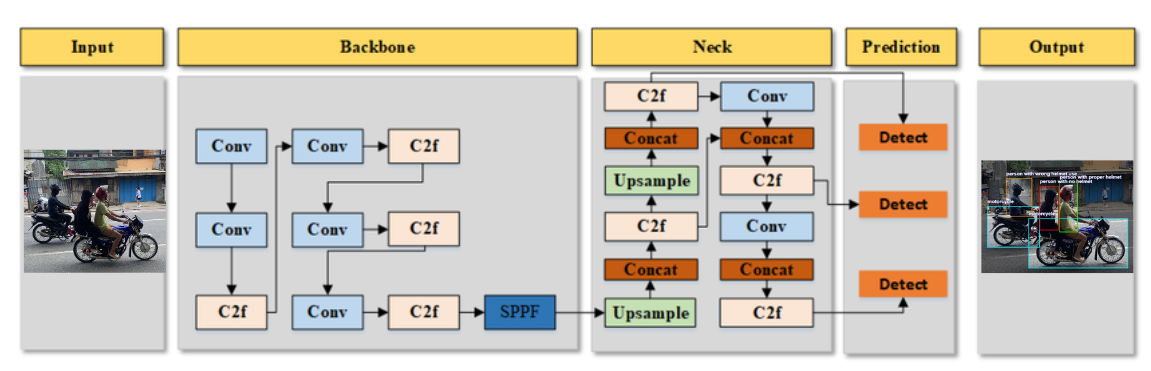
\includegraphics[width=0.85\textwidth]{figures/Fig 1.png} 
	\caption[ Yolov8 Object Detection Architecture]{Figure 1 illustrates the YOLOv8 architecture, where the input image is first resized and normalized, then passed through the backbone for feature extraction using convolutional layers and C2f blocks, followed by the neck that refines and fuses multi-scale features through concatenation and upsampling, and finally through a decoupled prediction head for separate classification and localization, producing bounding boxes and labels that are filtered using Non-Maximum Suppression to yield accurate and confident object detections.}
	\label{fig:firstFig}
\end{figure}

\section*{Detection Mechanism of Yolov8}

\subsection*{Bounding Box Prediction}

YOLOv8 predicts the center coordinates $(x_{pred}, y_{pred})$, width $(w_{pred})$, 
and height $(h_{pred})$ for each object within a grid cell.

The confidence score, used for evaluating bounding box accuracy, is given by the formula:

\[
Confidence = P_{object} \times IOU_{pred,truth}
\]

\subsection*{Class Probability Prediction}

YOLOv8 outputs a probability distribution across multiple object classes. 
For each bounding box, the network predicts the likelihood that it belongs 
to a particular class (e.g., helmet, rider, license plate).

\subsection*{\textit{Complete Intersection over Union (CIoU)}}

To optimize bounding box predictions, YOLOv8 utilizes the Complete Intersection over Union (CIoU) loss function, which improves upon the standard IoU by incorporating the overlap area, the distance between the center points of the predicted and ground truth boxes, and the consistency of their aspect ratios. This results in a more precise and reliable evaluation for object detection tasks.

Intersection over Union (IoU) is a key metric for evaluating object detection models, measuring the overlap between predicted and ground truth bounding boxes. The following figure illustrates IoU and its role in assessing detection accuracy, with an emphasis on YOLOv8’s enhanced approach.

\section*{\textbf{\textit{ YOLOv8 Object Detection Algorithm}}}
\begin{figure}[ht]
    \centering
	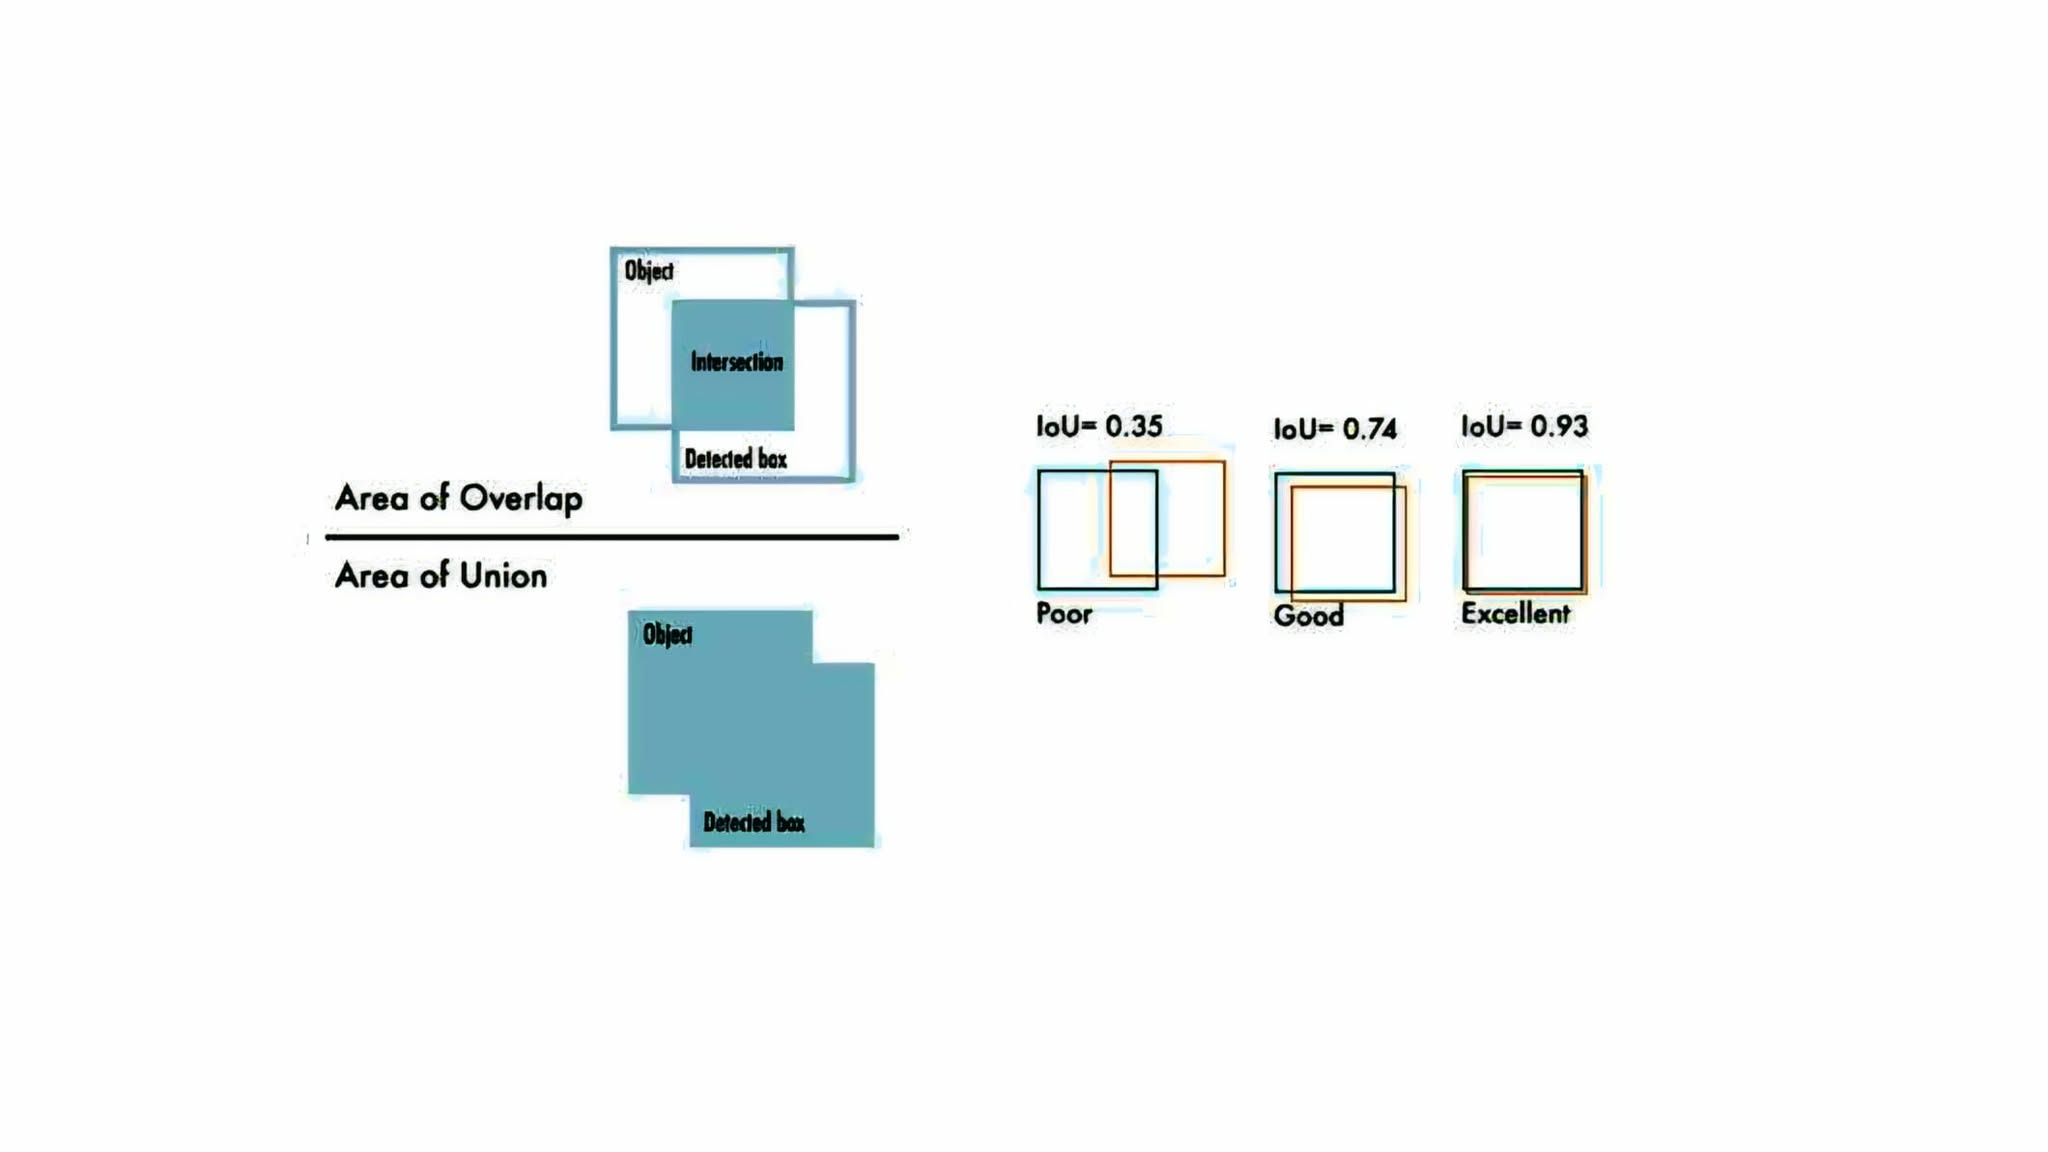
\includegraphics[width=0.85\textwidth]{figures/Fig 2.png} 
	\caption[ Intersection over Union ]{As illustrated in Figure 1, IoU is computed by dividing the overlapping area of two boxes by their total combined area, indicating how closely the predicted box aligns with the ground truth. The figure further demonstrates this concept through three examples showing IoU values of 0.35, 0.74, and 0.93, corresponding to poor, good, and excellent box alignment, respectively. YOLOv8 further enhances this evaluation by using Complete Intersection over Union (CIoU), which incorporates not only the overlap area but also the distance between box centers and the difference in aspect ratios. This leads to more accurate localization and robust object detection performance \cite{Terven2023}.}
	\label{fig:firstFig}
\end{figure}

\subsection*{Non-Maximum Suppression (NMS)}

YOLOv8 employs Non-Maximum Suppression (NMS) to efficiently eliminate redundant bounding boxes that predict the same object. After the model generates multiple bounding boxes, NMS ranks them according to their confidence scores, identifying how likely each box contains an object. The algorithm then selects the highest-scoring box and suppresses any overlapping boxes whose Intersection over Union (IoU) with the selected box exceeds a predefined threshold. This process ensures that each detected object is represented by only one bounding box, reducing clutter and improving the clarity of detection results. 

The following figure demonstrates how NMS improves detection clarity and reduces overlap.

\section*{\textbf{\textit{ YOLOv8 Object Detection Algorithm}}}
\begin{figure}[ht]
    \centering
	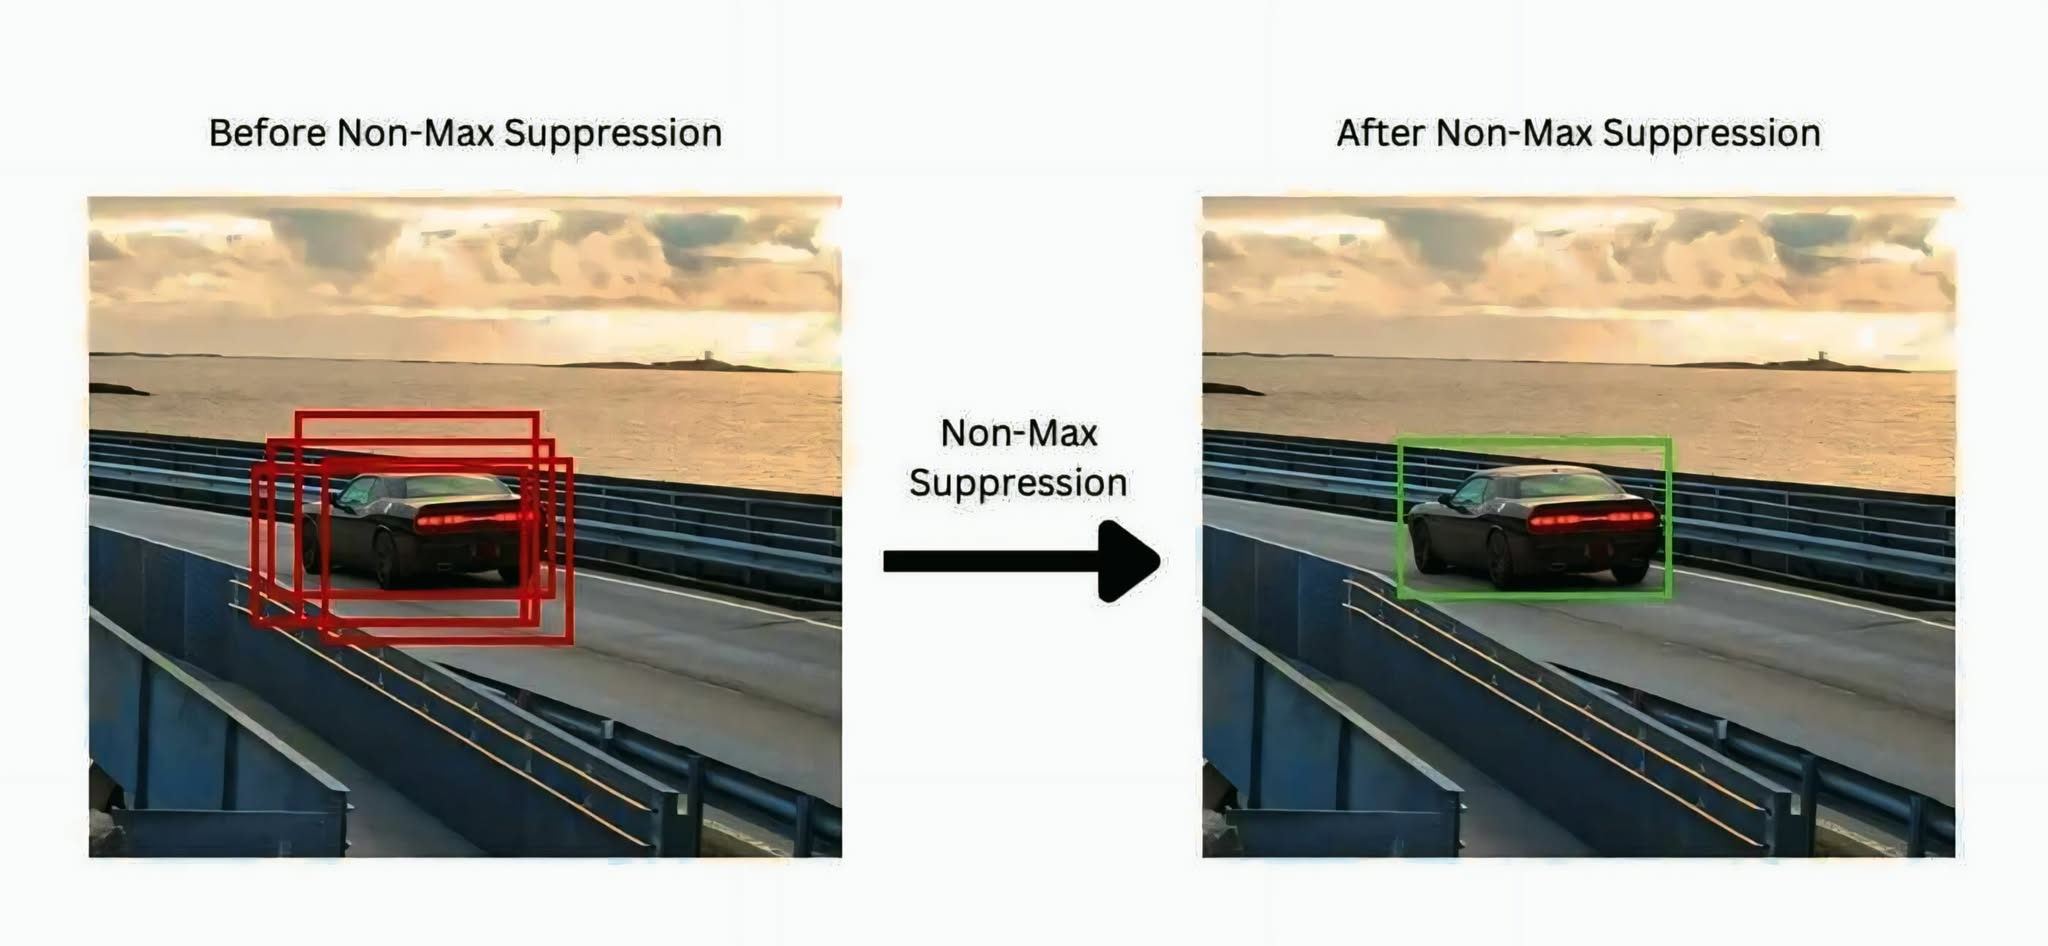
\includegraphics[width=0.85\textwidth]{figures/Fig 3.png} 
	\caption[ Example of Non-Maximum Suppression ]{Figure 3 effectively highlights the importance of Non-Maximum Suppression (NMS) in enhancing the quality of object detection results produced by YOLOv8. Without NMS, as seen in the left image, the model outputs numerous overlapping bounding boxes for a single object, which can negatively affect both the interpretability of results and the accuracy of object localization. The right image, post-NMS, shows a single, high-confidence bounding box, demonstrating the algorithm’s ability to reduce redundancy and improve detection clarity. This reduction in noise not only improves the precision of the model but also reduces computational complexity during post-processing. In our study, applying NMS was crucial in refining predictions, particularly in scenes with multiple or closely spaced objects. The figure provides clear visual evidence of how NMS contributes to the robustness and efficiency of the YOLOv8 algorithm.}
	\label{fig:firstFig}
\end{figure}

\section*{Materials and Statistical Tools/Evaluation Methods}

This section provides detailed information on the materials, statistical tools, and evaluation methods employed in the development and assessment of the Helmet Compliance Detection Using Computer Vision for Safer Roads. It includes the hardware and software components, the process followed to implement the prototype, the sampling technique, the statistical tests used for performance evaluation, and the methods employed for evaluating the prototype's effectiveness.

\
%=======================================================%
%%%%% Do not delete this part %%%%%%
\clearpage

\printbibliography[heading=subbibintoc, title={\texorpdfstring{\centering}{} Notes}]
\end{refsection}